\documentclass[12pt, letterpaper]{article}

\usepackage[utf8]{inputenc}
\usepackage{graphicx}
\usepackage{amsmath}

\graphicspath{ {images/}}

% Metadata
\title{Deep Work notes}
\author{Nenad Stojanovikj}
\date{November 2018}

\begin{document}

\begin{titlepage}
    \centering
    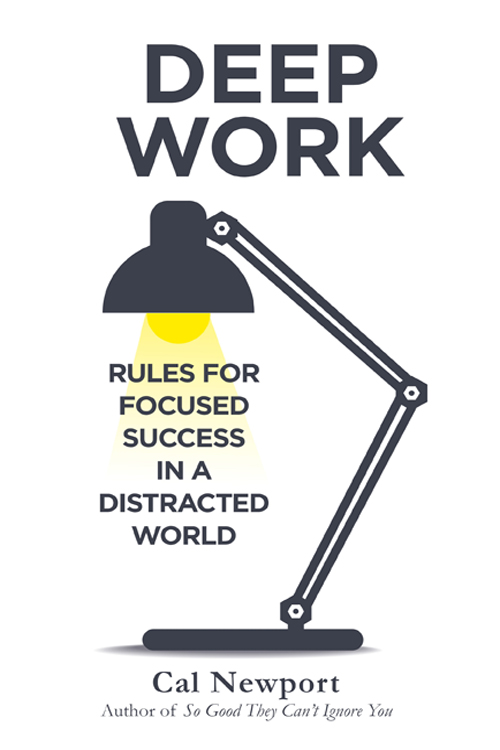
\includegraphics[width=0.20\textwidth]{cover}\par\vspace{1cm}
    {\scshape\LARGE Deep Work\par}
    {\scshape\small a book by Cal Newport\par}
    {\scshape\LARGE NOTES\par}
    \vspace{1cm}
    {\Large\itshape Nenad Stojanovikj\par}
    \vfill
    {\large \today\par}
    %\maketitle
    \thispagestyle{empty}
    \setcounter{page}{0}
\end{titlepage}

\tableofcontents
\break

\section*{Introduction}
\addcontentsline{toc}{section}{Introduction}

One of the most effective technique for immersing in deep work is isolating yourself for longer periods of time, where you can do work with no distractions.

Many famous people practiced this method. For example, the famous physicist Carl Jung created a tower in the middle of the woods just so he could work uninterrupted. Bill Gates used to go to a lakeside cottage two times a year, where he conducted his ``Think Weeks" - thinking big thoughts. Another example is Woody Allen, who wouldn't even touch a computer, but write everything on his typewriter. In 44 years, he wrote and directed 44 films.

\bigbreak
The Internet, and the \emph{Networking Tools} are very attractive distractions, which often find a way to get to us. Enough \emph{Shallow Work} will \emph{permanently} reduce our capacity to do \emph{Deep Work}.

\bigbreak
\textbf{Deep Work definition:} Professional activities performed in a state of distraction-free concentration that push your cognitive capabilities to their limit. These efforts create new value, improve your skill, and are hard to replicate.

\textbf{Shallow Work definition:} Non-cognitively demanding, logistical-style tasks, often performed while distracted. These efforts tend to not create much new value in the world, and are very easy to replicate.

\bigbreak
\textbf{The \emph{Deep Work} Hypothesis:} The ability to perform deep work is becoming increasingly rare at exactly the same time it is becoming increasingly \emph{valuable} in the current economy. As a consequence, the ones that cultivate this skill, and then make it the core of their working life, will thrive.

\bigbreak
\emph{Deep Work} is a skill that can be learned. With enough practice, everyone can produce good amount of quality work.

\break
\section*{The Idea}
\addcontentsline{toc}{section}{The Idea}
\subsection*{Deep Work Is Valuable}
\addcontentsline{toc}{section}{Deep Work Is Valuable}

Successful people belong to three categories.

\bigbreak\noindent\textbf{The High-Skilled Worker}

People who can work well with intelligent machines belong to this group. Working with voice recognition, robotics, data visualization, analytics, high speed communications, would classify you in this category.

The key question would be \emph{Are you good at working with intelligent machines or not?}

\bigbreak\noindent\textbf{The Superstar}

Being the \emph{best} in your profession would put you in this group.

% High-speed data networks and collaboration tools like e-mail and virtual meeting software have destroyed regionalism in many sectors of knowledge work. No longer you need to be in the same office space, employed as a full-time programmer.
This ``winner-take-all" behavior has been observed in a 1981 paper, by Sherwin Rosen. He labeled talent with the variable \emph{q} in his formulas, as a factor with \emph{imperfect substitution}, which he explained with the following sentence: ``Hearing a succession of mediocre singers does not add up to a single outstanding performance." You can't buy talent in bulk and combine it to reach the needed levels. There is a premium to being the best. If you are in a market, where the \emph{q} value of the performers is visible, everyone would be choosing the highest, even if the talent advantage of the best is \textit{slightly} better compared to the second.

\bigbreak\noindent\textbf{The Owner}

Having capital to invest in the new technologies that are driving the Great Restructuring would put you in this group. \emph{The book doesn't focus on this category.}

\subsection*{How to become a winner in the New Economy}
\bigbreak\noindent\textbf{Two \emph{core} abilities for thriving}
\begin{enumerate}
    \item The ability to quickly master hard things
    \item The ability to produce at an elite level, in terms of both quality and speed
\end{enumerate}

To join the group of those who can work well with intelligent machines, you need to hone your ability to master hard things. Because these technologies change rapidly, you must be able to master them quickly, again and again. This is not only applied to tech jobs, but any skill that you want to become master at.

Bottom line is, \emph{If you can't learn, you can't thrive.}

Now, looking at the second ability from the list: producing at an elite level. If you want to become a superstar, mastering the relevant skills is necessary, but not sufficient. You also must be able to ``sell'' (transform) that potential into tangible results that people will value. Many developers can program well, but leveraging that ability to provide something valuable to many people is what will build reputation.

The key idea from this ability is to understand that \emph{If you don't produce, you won't thrive.}

\bigbreak\textbf{The two described core abilities depend on your ability to perform deep work.}
If you haven't mastered this foundational skill, you will struggle to learn hard things, or produce at an elite level. The dependence of these abilities on deep work requires understanding of the science of learning, concentration and productivity.

\subsection*{Deep Work helps you quickly learn hard things}

\begin{quote}
Let your mind become a lens, thanks to the converging rays of attention; let your sould be all intent on whatever it is that is established in your mind as a dominant, wholly absorbing idea. \par\emph{--- Antonin-Dalmace Sertillanges}
\end{quote}

To learn requires intense concentration. A study in the 1970s found out that what separated the experts (in many different fields) from everyone else, was the use of \emph{deliberate practice}. Deliberate practice requires two things:
\begin{enumerate}
    \item Your full attention focused tightly on a specific skill you are trying to improve, or an idea you are trying to master
    \item You receive feedback so you can correct your approach to keep your attention exactly where it's most productive
\end{enumerate}

While regular practice might include mindless repetition, deliberate practice requires full attention and is conducted with the specific goal of improving performance.
Deliberate practice cannot coexist alongside distraction, as it requires uninterrupted concentration.

The science behind deliberate practice is that, by focusing intensely on a specific skill, you are forcing the specific relevant circuit to fire, again and again, in isolation. The repetitive use of the specific circuit triggers cells, that wrap layers of myelin around the neurons in the circuits --- effectively cementing the skill.

\subsection*{Deep Work helps you produce at an elite level}
To produce at an elite level, you need to produce. The time allocation for producing has to be carefully scheduled in order to have the best productivity.

The ``law of productivity'' is as follows:

\begin{equation*}
    \text{High-QualityWorkProduced} = \text{TimeSpent} \times \text{IntensityOfFocus}
\end{equation*}

Doing multitasking is dramatically reducing the intensity of the focus, which in turn lowers the productivity. Whenever a task is switched, it is followed by ``attention residue'' from the previous task. This residue still thinks about the old task, even though we work on a different task. Focusing on one task and finishing it minimizes the attention residue when we change tasks.

\section*{Deep Work is rare}

With many tech companies embracing the open-office concept, rapid communication through inter-company chat applications, active presence on social mediums it's hard to do deep work, when all of these trends actively \emph{decrease} one's ability to go deep.

\subsubsection*{The Metric Black Hole}
Measuring the cost of distractions can be very hard, because it's hard to measure one's contribution to the firm's output.

\subsubsection*{The Principle of Least Resistance}

A survey found out individuals that practice the \emph{culture of connectivity}, where one is expected to read and respond to communication quickly, spent around twenty, to twenty-five hours a week \emph{outside the office} believing that it's important to answer \emph{any} e-mail or instant message an hour of it's arrival.

A researcher conducted an experiment to test this claim. She forced each person from the team to take one working day without any connectivity to anyone inside or outside the company. After some time, the team members found more enjoyment in their work, better communication between themselves, more learning, and most importantly, a better product delivered to the client.

\textbf{The Principle of Least Resistance:} In a business setting, without clear feedback on the impact of various behaviors to the bottom line, we will tend toward behaviors that are easiest in the moment.

This principle supports work cultures that save us from the short term discomfort of concentration and planning, at the expense of long-term satisfaction and the production of real value. By doing so, this principle drives us toward shallow work in an economy that increasingly rewards depth.

Why does this happen? Because it's easier to do a shallow task instead of a deep one, which requires you to be focused on something for a certain period of time.

\subsubsection*{Business as a Proxy for Productivity}

In different areas, there are various measurement points that we can use to determine how productive we are. For example, as an academic researcher, your measurement question is ``Are you publishing important papers?''. This can be quantified as a single number that will represent your impact in your field. In some professions, you cannot quantify the productive work easily. This begs the question how can people know that you are working?

\textbf{Business as a Proxy for Productivity:} In the absence of clear indicators of what is means to be productive and valuable in their jobs, many knowledge workers turn back toward an industrial indicator of productivity: doing lots of stuff in a visible manner.

\break

\section*{Deep Work is Meaningful}

Finding a meaning in your profession gives motivation and satisfaction in what you do.

In craftsmanship professions, to be good, you must spend most of your time in state of depth, because even a small slip of concentration could ruin dozens of hours of effort. The connection between deep work, and good life is familiar and widely accepted when considering the world of craftsman.

In knowledge work, this connection is muddied. Craftsmen tackle professional challenges that are simple to define, but very hard to execute perfectly --- this is a useful imbalance when seeking purpose. Knowledge work exchanges this clarity for ambiguity. Another issue is the sheer amount of attractive distractions that are tempting us with shallow work on the screen, in front of our eyes every day.

\subsubsection*{A Neurological Argument for Depth}

After a cancer diagnosis, science writer Winifred Gallagher took a spin on her views on life. She said ``The disease wanted to monopolize my attention, but as much as possible, I would focus on my life instead.'' She focused only on the good things in life, for example, movies, walks and a 6:30 martini.

Our brains construct our worldview based on \emph{what we pay attention to}. If you focus on a cancer diagnosis, you and your life become unhappy and dark, but if you focus instead on an evening martini, you and your life become more pleasant --- even though the circumstances in both scenarios are the same.

\begin{quote}
    \emph{Who you are, what you think, feel, and do, what you love --- is the sum of what you focus on. --- Winifred Gallagher}
\end{quote}

\subsubsection*{A Psychological Argument for Depth}

An experiment was conducted, where selected individuals would have a pager with them, and this pager would beep randomly few times during the day. The individuals would have to report what they were doing, and how they felt. The conclusion was that, the best moments usually occur when a person's body or mind is stretched to its limits in a voluntary effort to accomplish something difficult and worthwhile. This mental state is called \emph{flow}.

People often assume that relaxation makes them happy. We want to work less, and spend more time in leisure activities. But the research found out the following:

\begin{quote}
    Ironically, jobs are actually easier to enjoy than free time, because like flow activities they have built-in goals, feedback rules, and challenges, all of which encourage one to become involved in one's work, to concentrate and lose oneself in it. Free time, on the other hand, is unstructured and requires much greater effort to be shaped into something that can be enjoyed.
\end{quote}

\end{document}
